\documentclass[11pt]{article}
\usepackage[T1]{fontenc}
\usepackage{lmodern}
\usepackage[letterpaper,margin=0.95in]{geometry}
\usepackage{amsmath,amssymb,amsthm,mathtools,booktabs,tabularx,graphicx,microtype}
\usepackage[hidelinks]{hyperref}
\usepackage{fancyhdr}
\pagestyle{fancy}\fancyhf{}\fancyhead[L]{\small Finite-kernel ratios and readout convergence}\fancyhead[R]{\small Section 3 research note 2}\fancyfoot[C]{\thepage}
\setlength{\headheight}{14pt}\setlength{\emergencystretch}{2em}
\allowdisplaybreaks[2]
\title{Why small tanh slopes make readout gradient descent slow\\[4pt]\large Two-sided finite-network eigenvalue bounds and training time}
\author{}\date{Section 3 research note 2 --- 25 September 2026}
\begin{document}\maketitle
An accurate readout can exist even when ordinary gradient descent needs an impractical number of updates to find it. We study a tanh network with frozen centers and a common slope \(\gamma\). The argument has four steps: derive gradient descent's dependence on normalized kernel eigenvalues; replace the center sum by an explicit integral; bound the finite eigenvalues above and below using that integral and controlled corrections; and substitute the ratio interval into the target's error formula. Small gamma attenuates high frequencies in the integral. The finite-network bounds quantify the resulting small learning rates in the geometry we test.

The mechanism is that increasing gamma restores higher-frequency contributions by much larger factors than lower-frequency contributions. The proof expresses this through a positive Fourier integral, then keeps the effects of the finite center grid and halo explicitly. The theorem is an interval evaluated at each gamma, with no starting gamma or reference eigenvalue. Its upper ratio endpoints give necessary training times; its lower endpoints give sufficient times. This does not assert that every actual ratio increases for every geometry. The mathematical inequalities are exact; the figures are checked floating-point evaluations, not interval-arithmetic certificates. All errors and times concern the specified training samples and raw readout coordinates.

\section{Frozen geometry: the normalized eigenvalues determine convergence}

For \(m\ge2\) training inputs \(x_a\) and \(W\) tanh centers \(c_j\), including halo centers, define \(B_\gamma\in\mathbb R^{m\times(W+1)}\) by

\[
(B_\gamma)_{aj}=m^{-1/2}\tanh(\gamma(x_a-c_j)),
\qquad (B_\gamma)_{a0}=m^{-1/2}.
\]

Column zero is the bias feature. With \(y_a=f(x_a)/\sqrt m\), the readout coefficients \(v\) minimize \(L(v)=\tfrac12\|B_\gamma v-y\|^2\). Geometry is fixed throughout training. Writing \(r_n=B_\gamma v_n-y\), an ordinary gradient descent update gives

\[
\begin{aligned}
v_{n+1}&=v_n-\eta_\gamma B_\gamma^\top r_n,\\
r_{n+1}&=B_\gamma(v_n-\eta_\gamma B_\gamma^\top r_n)-y
=(I-\eta_\gamma K_\gamma)r_n,
\qquad K_\gamma=B_\gamma B_\gamma^\top.
\end{aligned}
\tag{1}
\]

Starting at \(v_0=0\) gives \(r_0=-y\). Order the kernel eigenvalues as \(\lambda_1\ge\cdots\ge\lambda_m\ge0\), with orthonormal eigenvectors \(u_i\). Throughout, use

\[
\eta_\gamma=\frac1{2\lambda_1(\gamma)},
\qquad
\rho_i(\gamma)=\frac{\lambda_i(\gamma)}{\lambda_1(\gamma)}.
\]

Each eigenvector component then satisfies

\[
u_i^\top r_n=-u_i^\top y\,(1-\rho_i/2)^n.
\tag{2}
\]

Multiplying the entire kernel by a scalar leaves these factors unchanged. What matters is the ratio \(\rho_i\), together with the target component along \(u_i\). Define its squared-norm fraction by \(p_i(\gamma)=|u_i(\gamma)^\top y|^2/\|y\|^2\). The exact relative training error is

\[
\boxed{
E_\gamma(n)^2:=\frac{\|r_n\|^2}{\|y\|^2}
=\sum_{i=1}^m p_i(\gamma)(1-\rho_i(\gamma)/2)^{2n}.
}
\tag{3}
\]

The weights sum to one. A zero eigenvalue contributes an irreducible component; a small positive eigenvalue contributes a representable component that decays slowly. The next two sections bound the ratios. Section 4 uses those bounds in (3), retaining the actual target weights.

\section{A center integral separates the explicit matrix from the finite corrections}

The actual kernel entries are

\[
(K_\gamma)_{ab}=\frac1m\left[1+\sum_{j=1}^{W}g_{ab}(c_j)\right],
\quad
g_{ab}(c)=\tanh(\gamma(x_a-c))\tanh(\gamma(x_b-c)).
\]

We now consider the continuous version \(K_\gamma^{\mathrm{int}}\), taking an integral inner product over functions of the center coordinate \(c\). The sample locations remain fixed. Assume consecutive lattice centers with spacing \(h\); their cells cover \(I_c=[c_1-h/2,c_W+h/2]\), of length \(Wh\). Then

\[
(K_\gamma^{\mathrm{int}})_{ab}
=\frac1m\left[1+\frac1h\int_{I_c}g_{ab}(c)\,dc\right],
\qquad E_\gamma^{\mathrm{grid}}=K_\gamma-K_\gamma^{\mathrm{int}}.
\tag{4}
\]

The factor \(1/h\) matches the center density. Writing \(g_{ab}=1-(1-g_{ab})\), the constant integral gives \(Wh\), while the whole-line deficit has the explicit value

\[
\int_{\mathbb R}(1-g_{ab}(c))\,dc
=2d_{ab}\coth(\gamma d_{ab}),\qquad d_{ab}=x_a-x_b.
\]

At \(d_{ab}=0\), the value is \(2/\gamma\). Restoring the deficit outside \(I_c\) gives the exact decomposition

\[
\boxed{
K_\gamma=
\underbrace{\frac{W+1}{m}\mathbf1\mathbf1^\top
-\frac2{hm}[d_{ab}\coth(\gamma d_{ab})]_{a,b}}_{K_\gamma^{(0)}}
+E_\gamma^{\mathrm{halo}}+E_\gamma^{\mathrm{grid}},
}
\tag{5}
\]

where \((E_\gamma^{\mathrm{halo}})_{ab}=(hm)^{-1}\int_{\mathbb R\setminus I_c}(1-g_{ab}(c))\,dc\). Appendix A derives the integral.

The explicit matrix has a constant rank-one term and a term depending only on the separation \(x_a-x_b\). On equally spaced samples, its entries are constant along each diagonal: this is the Toeplitz structure. It is not a diagonal matrix. The corrections retain the dependence on the finite center interval and the discrete center lattice. We do not assume Fourier waves are eigenvectors of the sampled matrix.

\begin{figure}[htbp]\centering
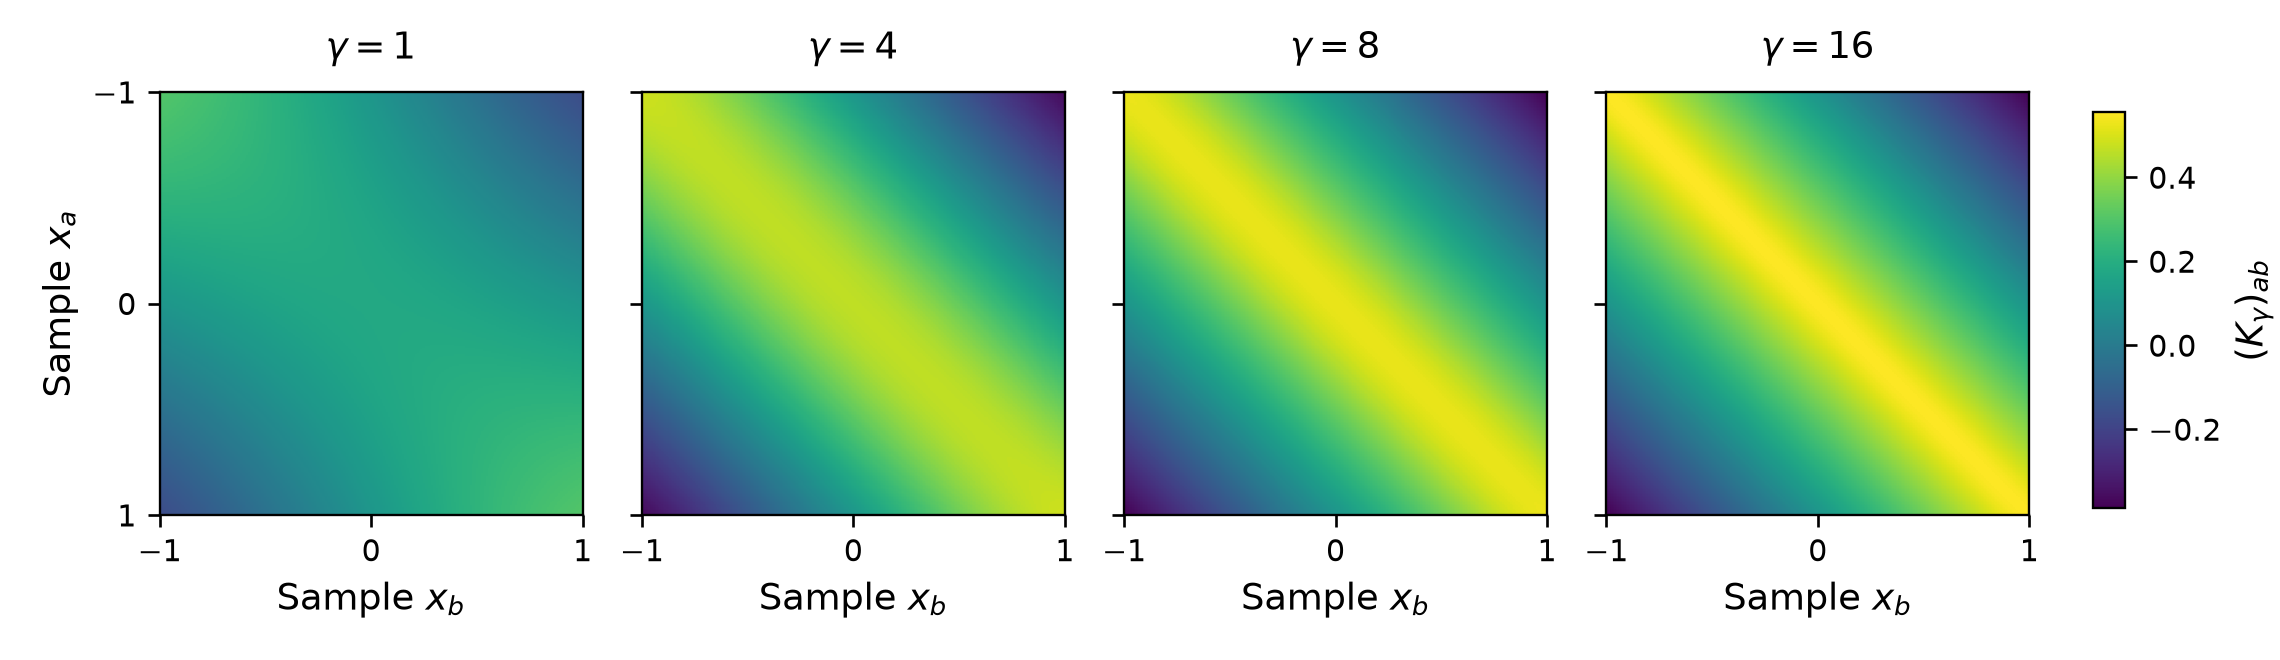
\includegraphics[width=\linewidth]{figures/finite_kernels.png}
\caption{Actual matrices \(K_\gamma=B_\gamma B_\gamma^\top\) at \(\gamma=1,4,8,16\), using identical samples and centers and a common color scale. The separation-dependent term produces the diagonal bands. These are full finite matrices, including the bias, grid, and halo contributions.}
\end{figure}

\section{The Fourier integral gives a two-sided finite-network ratio bound}

\subsection{How gamma enters the integral matrix}

Tanh is a step averaged with the density \(\rho_\gamma^{\mathrm{av}}(x)=\gamma\operatorname{sech}^2(\gamma x)/2\):

\[
(\rho_\gamma^{\mathrm{av}}*\operatorname{sgn})(x)
=2\int_{-\infty}^{x}\rho_\gamma^{\mathrm{av}}(t)\,dt-1
=\tanh(\gamma x).
\]

With \(\widehat f(\omega)=\int f(x)e^{-i\omega x}\,dx\), convolution multiplies the transform by

\[
M_\gamma(\omega)=\widehat{\rho_\gamma^{\mathrm{av}}}(\omega)
=\frac{z}{\sinh z},\qquad z=\frac{\pi|\omega|}{2\gamma},
\qquad M_\gamma(0)=1.
\tag{6}
\]

This averaging acts in both inputs of the feature-product kernel: its two-input Fourier transform is multiplied by \(M_\gamma(\omega)M_\gamma(\omega')\) relative to the step kernel. Thus small gamma suppresses high-frequency variation in the kernel entries. The next identity connects that suppression to eigenvalues, without identifying Fourier waves with eigenvectors.

Let \(Q\in\mathbb R^{m\times(m-1)}\) have orthonormal columns spanning vectors whose entries sum to zero: \(Q^\top Q=I\), \(Q^\top\mathbf1=0\). This removes one constant direction for the calculation; it places no assumption on the actual eigenvectors. For \(t_\gamma(c)=(\tanh(\gamma(x_a-c)))_{a=1}^{m}\), define

\[
H_\gamma:=\frac1{hm}\int_{\mathbb R}
Q^\top t_\gamma(c)t_\gamma(c)^\top Q\,dc
=Q^\top K_\gamma^{(0)}Q.
\]

The constant tails cancel after projection, so this integral is finite. For any vector \(v\in\mathbb R^{m-1}\), set \(u=Qv\). The following three steps explain its quadratic form:

\[
g_\gamma(c):=\sum_a u_a\tanh(\gamma(c-x_a)),
\qquad v^\top H_\gamma v=\frac1{hm}\int |g_\gamma(c)|^2\,dc;
\]
\[
\widehat g_\gamma(\omega)
=M_\gamma(\omega)\frac{2}{i\omega}
\sum_a u_a e^{-i\omega x_a};
\]
\[
\boxed{
v^\top H_\gamma v
=\frac2{\pi hm}\int_{\mathbb R}
\frac{M_\gamma(\omega)^2}{\omega^2}
\left|\sum_a (Qv)_a e^{-i\omega x_a}\right|^2\,d\omega.
}
\tag{7}
\]

The middle line follows by differentiating the sum of steps; the last is Parseval's identity. Here \(u_a=(Qv)_a\) is the entry of a sample-space vector, not a readout coefficient. The apparent singularity at zero is removable because \(\sum_a u_a=0\). Appendix B gives the details.

For a fixed \(v\), all gamma dependence in (7) is in \(M_\gamma^2\), and every contribution is nonnegative. If \(v\) is a unit eigenvector of \(H_\gamma\), this integral is its eigenvalue. Increasing gamma increases the integral for every fixed vector, so \(H_{\gamma_b}\succeq H_{\gamma_a}\) for \(\gamma_b\ge\gamma_a\). The minimum--maximum characterization then proves that every ordered eigenvalue of \(H_\gamma\) is nondecreasing, even though its eigenvectors can change.

\subsection{Why different eigenvalues can grow by very different factors}

The important fact is not just that the multiplier increases. Its increase is much larger at higher frequencies. Doubling gamma gives the exact identity
\[
\boxed{\frac{M_{2\gamma}(\omega)^2}{M_\gamma(\omega)^2}
=\cosh^2\!\left(\frac{\pi|\omega|}{4\gamma}\right).}
\tag{7a}
\]
For \(|\omega|\ll\gamma\), this factor is close to one. For \(|\omega|\gg\gamma\), it grows as \(\tfrac14 e^{\pi|\omega|/(2\gamma)}\). Small gamma therefore does not shrink every part of the matrix by the same amount, and increasing gamma does not restore every part by the same amount.

For \(v^\top H_\gamma v>0\), divide the nonnegative integrand in (7) by its integral and call the resulting frequency density \(w_{\gamma,v}(\omega)\). Thus \(w_{\gamma,v}\) integrates to one and records which frequencies contribute to the quadratic form of the chosen vector. Then
\[
\boxed{\frac{v^\top H_{2\gamma}v}{v^\top H_\gamma v}
=\int_{\mathbb R}\cosh^2\!\left(\frac{\pi|\omega|}{4\gamma}\right)
 w_{\gamma,v}(\omega)\,d\omega.}
\tag{7b}
\]
Low-frequency contributions change little; higher-frequency contributions receive larger multiplicative gains. The direction's total gain is their weighted average in (7b). A substantial weight at higher frequencies therefore forces a larger gain; Appendix B makes this lower bound explicit. This connects Fourier suppression to unequal changes in quadratic forms without requiring a Fourier wave to be an eigenvector.

Equation (7b) holds the vector fixed for a finite change. It would be incorrect simply to identify its two sides with the same ranked eigenvalue at both gammas. To account for changing eigenvectors, take a simple positive eigenvalue of \(H_\gamma\) with unit eigenvector \(v_i(\gamma)\). The exact local version is
\[
\boxed{\frac{d\log\lambda_i(H_\gamma)}{d\log\gamma}
=\int_{\mathbb R}2(z\coth z-1)\,w_{\gamma,v_i}(\omega)\,d\omega,
\qquad z=\frac{\pi|\omega|}{2\gamma}.}
\tag{7c}
\]
The factor \(2(z\coth z-1)\) increases strictly with frequency. It is approximately \(\pi^2\omega^2/(6\gamma^2)\) at low frequency and \(\pi|\omega|/\gamma-2\) at high frequency. Appendix B derives (7a)--(7c), including the cancellation of eigenvector-derivative terms, and gives the exact counterpart for the actual finite kernel with all corrections retained.

A small eigenvalue alone does not establish that its frequency weight is high: dependencies among features can also produce small eigenvalues. In the modes examined here, the existing frequency integrals test this association directly. For example, at gamma 16, about 96.43\% of the integral weight of the actual rank-32 eigenvector is above \(8\pi\). The Fourier weighted average evaluated on its centered component, as in (B5), is 6.90227; its actual finite-kernel logarithmic eigenvalue growth is 6.90230. The corresponding growth of the largest eigenvalue is only 0.01096. The subtraction of these two growth rates gives 6.89133 for the normalized rank-32 ratio. Appendix B reports the other checked modes and the precise finite-kernel accounting. These are saved numerical diagnostics, not an assumption that eigenvalue rank always orders frequency.

\subsection{What the largest-eigenvalue normalization contributes}

The ratio can improve only if the smaller eigenvalue grows by a larger factor than the largest one. We therefore bound the denominator as well. With \(e=\mathbf1/\sqrt m\), the finite features give
\[
\ell_\gamma:=e^\top K_\gamma e
=1+\sum_{j=1}^{W}\left[\frac1m\sum_a\tanh(\gamma(x_a-c_j))\right]^2
\le\lambda_1(K_\gamma)\le W+1.
\tag{7d}
\]
The upper bound follows because every feature entry has magnitude at most one. The lower bound counts the squared average of each feature, together with the bias. It contains no high-frequency cancellation. Exterior centers, in particular, give almost constant columns once their tanhs saturate. A center at distance \(d_j>0\) outside the sample interval contributes at least \(\tanh^2(\gamma d_j)\) to \(\ell_\gamma\). Thus the denominator already has substantial contributions that do not require recovering a suppressed fine-scale variation.

These statements bound its scale; they do not by themselves prove that it is nearly constant on every gamma interval. For the geometry in this note, the saved values make that last point quantitative: from gamma 8 to 64, \(\lambda_1\) moves from 72.674 to 74.240, while \(\ell_\gamma\) moves from 66.823 to 68.316. Meanwhile the rank-26 ratio moves from \(1.487\times10^{-7}\) to \(8.357\times10^{-4}\). The large improvement is therefore not a uniform rescaling of the kernel. Appendix D proves (7d), gives its step-limit dependence on gamma, and derives a sharper upper bound \(L_\gamma\) than \(W+1\).

\subsection{What beta, delta, and tau actually are}

The integral \(H_\gamma\) uses a continuous, infinite line of centers. Our network has discrete centers in a finite interval. We correct those two differences before claiming a bound on its eigenvalues:
\[
\boxed{S_\gamma=H_\gamma+G_\gamma-T_\gamma,
\qquad \beta_i(\gamma)=\lambda_i(S_\gamma).}
\tag{8}
\]
Here \(G_\gamma\) adds the first \(p\) Fourier terms of the error from replacing the center integral by a center lattice. Their frequencies are \(2\pi k/h\), and their entries are explicit expressions in \(M_\gamma(2\pi k/h)\) and \(\coth(\gamma(x_a-x_b))\), given in Appendix C. The matrix \(T_\gamma\) subtracts the outer products of finitely many exterior lattice centers that are not present in the actual network. Each of its entries is a finite sum of products of the specified tanhs. Neither correction is fitted to the actual small eigenvalues.

Thus \(\beta_i\) is not a free parameter or a gamma-independent constant. It is the ordered eigenvalue of this explicitly constructed, corrected integral matrix at the current gamma. Its calculation still requires a matrix eigendecomposition. The explanation of its dependence on gamma is the Fourier integral plus the specified corrections; hiding that calculation behind the letter beta would not supply an explanation.

The other two quantities bound only the terms that we did not explicitly retain:
\begin{itemize}
\item \(\delta_\gamma\) bounds the remaining center-lattice Fourier terms in operator norm. The omitted frequencies start at \(2\pi(p+1)/h\).
\item \(\tau_\gamma\) bounds the remaining exterior-center outer products. They are positive semidefinite, so omitting them has a known sign.
\end{itemize}
For fixed sample positions, let \(\bar x\) be their mean. Choose a strip angle \(0<\vartheta<\pi/2\) for the analytic estimate, and let \(d_R,d_L>0\) be the distances from the sample interval to the first unretained exterior centers on the right and left. The bounds are explicit:
\[
\begin{aligned}
\delta_\gamma&=
\frac{8\gamma\|x-\bar x\mathbf1\|^2\sec^4\vartheta}{3hm}
\frac{e^{-2\pi\vartheta(p+1)/(\gamma h)}}
     {1-e^{-2\pi\vartheta/(\gamma h)}},\\
\tau_\gamma&=4\frac{e^{-4\gamma d_R}+e^{-4\gamma d_L}}
                         {1-e^{-4\gamma h}}.
\end{aligned}
\tag{8a}
\]
The strip angle is a choice in the proof, not a model parameter. Appendix C derives these expressions. Larger gamma makes the uncomputed lattice tail harder to neglect at fixed \(p\), so more lattice terms may be required. It makes distant exterior centers easier to neglect, because their projected constant tails decay faster. The two allowances therefore do not both decrease with gamma. We choose the truncation counts to make their remainder small enough for the eigenvalue being studied; the retained corrections remain in \(S_\gamma\).

Writing the unretained lattice matrix as \(R_\gamma\), with \(\|R_\gamma\|\le\delta_\gamma\), and the unretained exterior matrix as \(T_{\mathrm{tail},\gamma}\), with \(0\preceq T_{\mathrm{tail},\gamma}\preceq\tau_\gamma I\), the exact relation is
\[
Q^\top K_\gamma Q=S_\gamma+R_\gamma-T_{\mathrm{tail},\gamma}.
\]
Consequently
\[
S_\gamma-(\delta_\gamma+\tau_\gamma)I
\preceq Q^\top K_\gamma Q
\preceq S_\gamma+\delta_\gamma I.
\tag{9}
\]
This is why delta and tau enter the theorem with those signs. They are proved remainders, not adjustable offsets that make the curves agree.

\textbf{Theorem 1 (finite-network eigenvalue and ratio interval).} Suppose the centers lie on a lattice of spacing \(h\), the common slope is positive, and \(S_\gamma\) is constructed by (8), with the explicit remainders (8a) derived in Appendix C. Then (9) holds. Let \(0<\ell_\gamma\le\lambda_1(K_\gamma)\le L_\gamma\). For \(2\le i\le m-1\), define

\[
\underline\lambda_i=[\beta_i-\delta_\gamma-\tau_\gamma]_+,
\qquad
\overline\lambda_i=\beta_{i-1}+\delta_\gamma,
\quad [t]_+=\max(t,0).
\]

Then

\[
\boxed{
\begin{gathered}
\underline\lambda_i\le\lambda_i(K_\gamma)\le\overline\lambda_i,\\
\underline\rho_i:=\frac{\underline\lambda_i}{L_\gamma}
\le\rho_i\le
\min\!\left\{1,\frac{\overline\lambda_i}{\ell_\gamma}\right\}
=:\overline\rho_i.
\end{gathered}
}
\tag{10}
\]

For \(i=m\), use \(\underline\lambda_m=0\) and \(\overline\lambda_m=\beta_{m-1}+\delta_\gamma\). Set \(\underline\rho_1=\overline\rho_1=1\). Known zero eigenvalues can be assigned both endpoints zero. These bounds depend only on the current gamma and geometry, not on a reference slope or old eigenvectors.

The proof is short once (9) is established. Its eigenvalues differ from \(\beta_i\) by the indicated allowances. Removing one dimension gives

\[
\lambda_i(K_\gamma)\ge\lambda_i(Q^\top K_\gamma Q),
\qquad
\lambda_i(K_\gamma)\le\lambda_{i-1}(Q^\top K_\gamma Q).
\]

Combining these inequalities gives the different indices in (10). Dividing the lower numerator by an upper denominator, and the upper numerator by a lower denominator, proves the ratio interval. In particular, no finite eigenvector is assumed to have zero mean. We may always take \(\ell_\gamma=1,L_\gamma=W+1\); the plots use sharper feature-average and block bounds from Appendix D, without using the actual small eigenvalues.

\begin{figure}[htbp]\centering
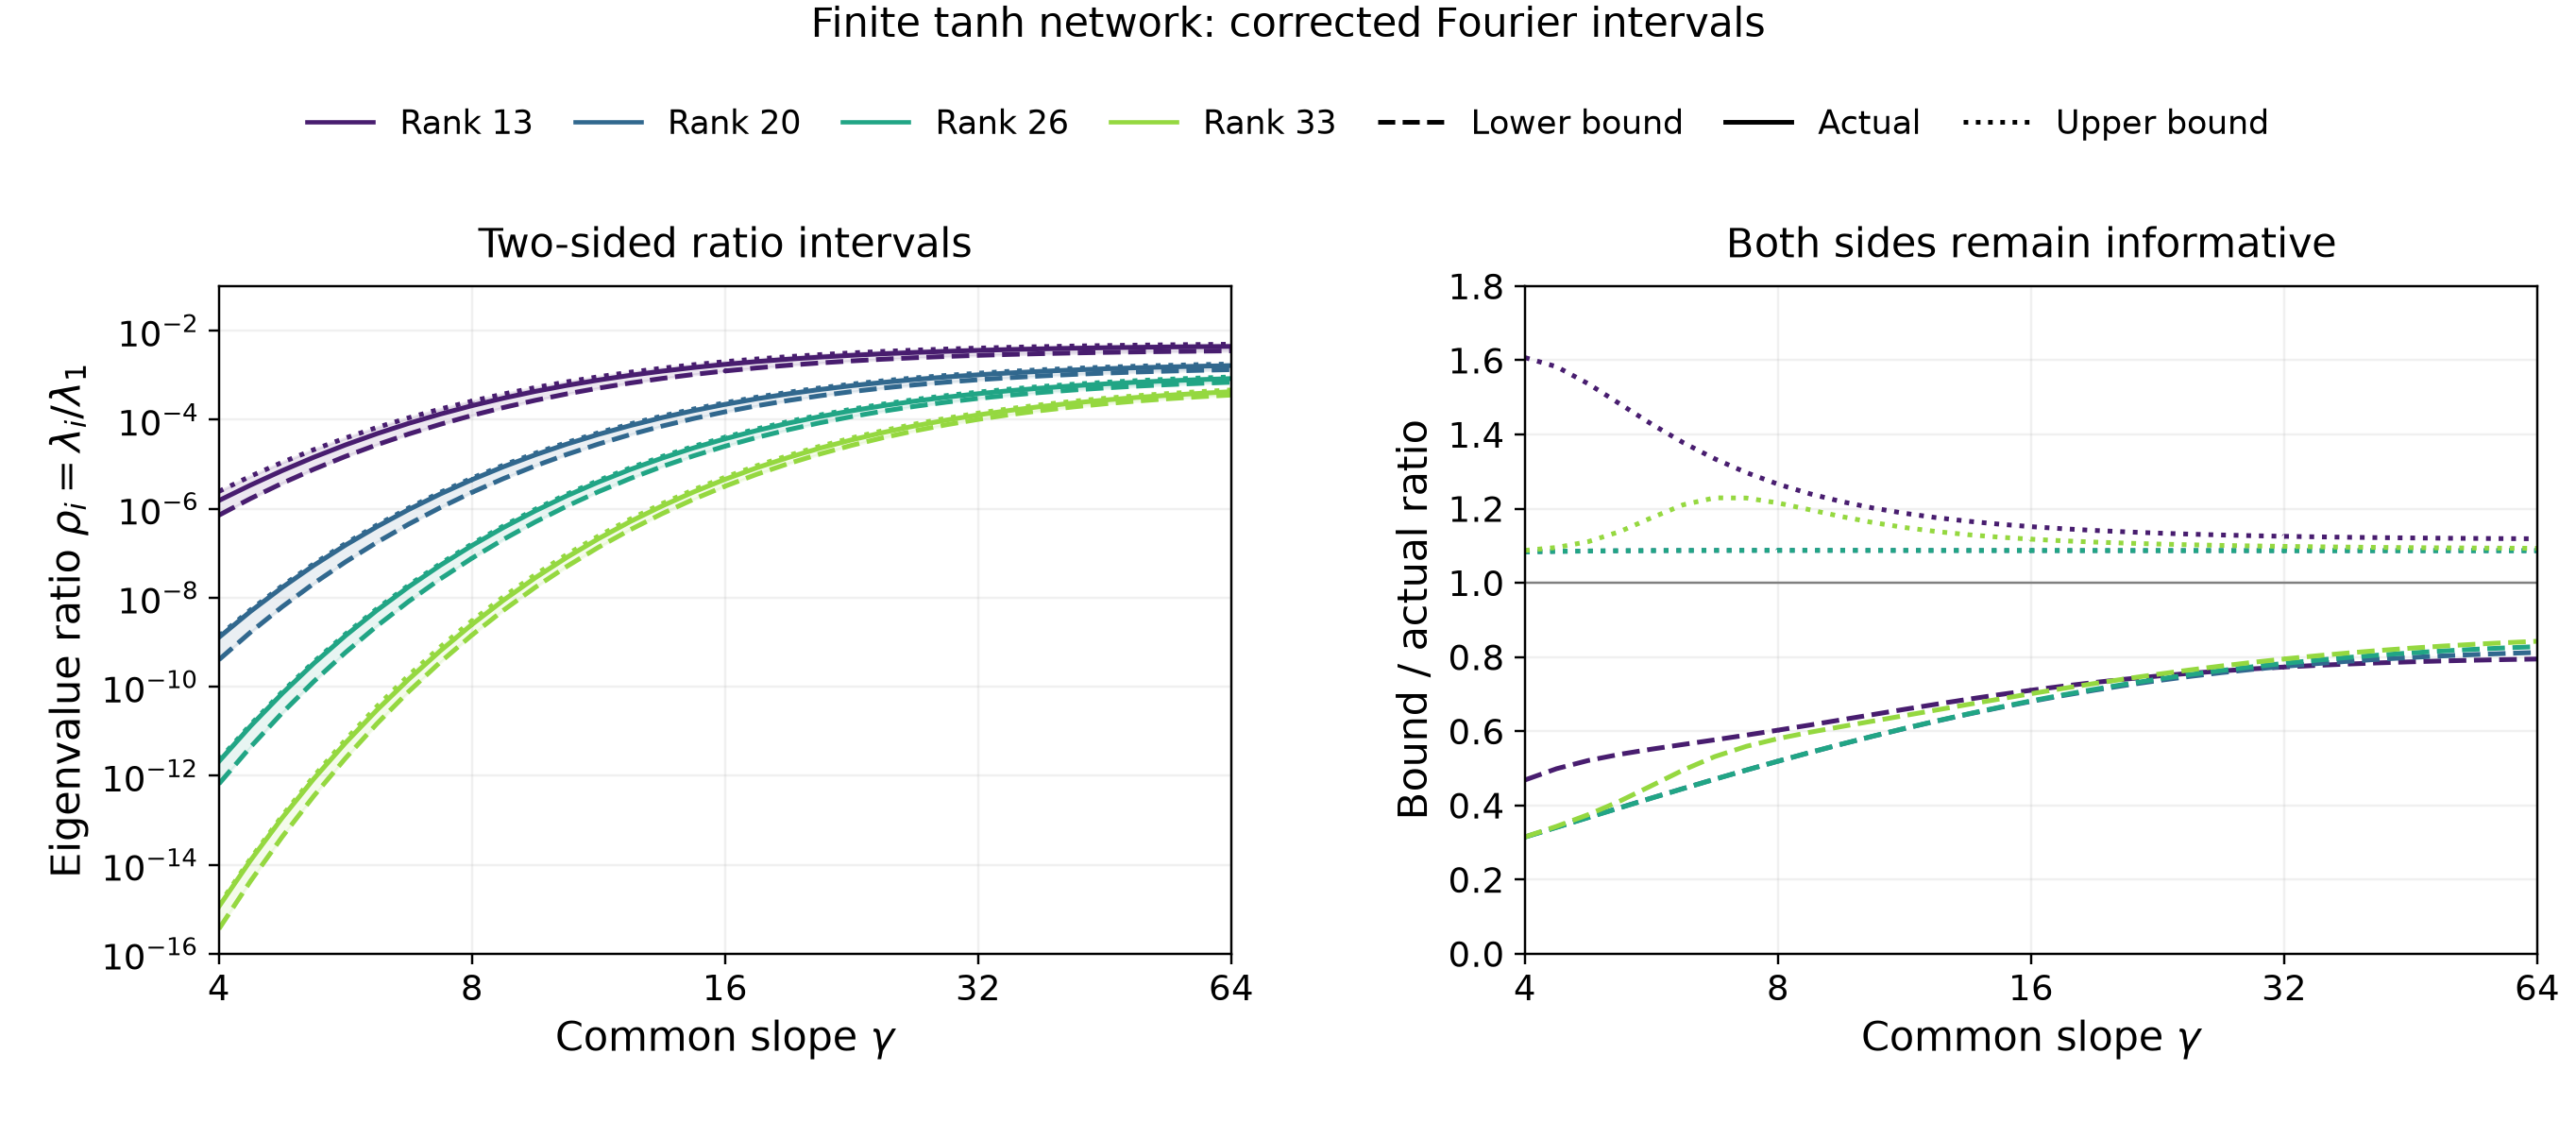
\includegraphics[width=\linewidth]{figures/ratio_intervals.png}
\caption{Actual finite-kernel ratios and the two endpoints from (10), at fixed centers and samples. Each color denotes an eigenvalue rank; solid lines are actual ratios, dashed lines the lower endpoints, and dotted lines the upper endpoints. The companion panel displays bound divided by actual ratio. These are single-gamma calculations, not comparisons anchored to an earlier spectrum. Numerical evaluations and their checks are described in Appendix F.}
\end{figure}

\begin{samepage}
For rank 26 in the default geometry, the evaluated intervals are:

\begin{center}\small\begin{tabularx}{\linewidth}{lXXX}
\toprule
\(\gamma\) & Lower ratio endpoint & Actual ratio & Upper ratio endpoint \\
\midrule
4 & \(6.562\times10^{-13}\) & \(2.088\times10^{-12}\) & \(2.262\times10^{-12}\) \\
8 & \(7.719\times10^{-8}\) & \(1.487\times10^{-7}\) & \(1.617\times10^{-7}\) \\
16 & \(2.532\times10^{-5}\) & \(3.715\times10^{-5}\) & \(4.039\times10^{-5}\) \\
64 & \(6.919\times10^{-4}\) & \(8.357\times10^{-4}\) & \(9.081\times10^{-4}\) \\
\bottomrule\end{tabularx}\end{center}
\end{samepage}

For gamma 4 and 8, the lower endpoint at 8 exceeds the upper endpoint at 4 by more than four orders of magnitude. Once endpoints are validly enclosed, the test
\[
\underline\rho_i(\gamma_b)>\overline\rho_i(\gamma_a)
\quad\Longrightarrow\quad
\rho_i(\gamma_b)>\rho_i(\gamma_a)
\tag{10a}
\]
proves an actual finite-ratio increase. It needs no assumption about unchanged eigenvectors or the sign of correction derivatives. The displayed values pass this test numerically for the stated geometry. Each endpoint is still calculated independently from its own gamma; there is no reference spectrum in the bound.

Equations (7a)--(7c) explain why removing Fourier suppression can produce a much larger multiplicative gain for the relevant small eigenvalues. Equations (8)--(10) check whether the finite lattice, halo, and normalization preserve that gain. These are different jobs. An analytic matrix-order statement for \(H_\gamma\) does not make the finite normalized ratios monotone automatically. Appendix E retains a counterexample, so the conclusion is the proved interval test and its checked evaluations, not an unsupported universal monotonicity claim.

\section{The ratio interval bounds both the error and the required number of steps}

For \(0\le\rho\le1\), the factor \((1-\rho/2)^{2n}\) decreases as \(\rho\) increases. Substituting the endpoints of (10) into (3) therefore gives

\[
\begin{aligned}
\underline E_\gamma(n)^2
&:=\sum_{i=1}^{m}p_i(\gamma)(1-\overline\rho_i(\gamma)/2)^{2n},\\
\overline E_\gamma(n)^2
&:=\sum_{i=1}^{m}p_i(\gamma)(1-\underline\rho_i(\gamma)/2)^{2n},
\end{aligned}
\]
\[
\boxed{\underline E_\gamma(n)^2\le E_\gamma(n)^2\le\overline E_\gamma(n)^2.}
\tag{11}
\]

Both sums use the same actual finite-network weights \(p_i(\gamma)\). We do not replace them by eigenvector weights from \(H_\gamma\) or \(S_\gamma\). The ratio theorem is target-independent; applying it to a particular target still requires its projections, or justified bounds on their energy.

The lower curve says how much error must remain: if \(\underline E_\gamma(n)>\epsilon\), no iterate up to step \(n\) can have reached tolerance. The upper curve says how much error can remain: if \(\overline E_\gamma(n)\le\epsilon\), the true curve has reached tolerance by that step. Define the first integer crossings

\[
\underline n_\epsilon=\min\{n\ge0:\underline E_\gamma(n)\le\epsilon\},
\qquad
\overline n_\epsilon=\min\{n\ge0:\overline E_\gamma(n)\le\epsilon\},
\]

with the minimum of an empty set equal to \(+\infty\). Then

\[
\boxed{\underline n_\epsilon(\gamma)\le n_\epsilon(\gamma)\le\overline n_\epsilon(\gamma).}
\tag{12}
\]

The two eigenvalue bounds have different jobs: upper ratios give a necessary time, while lower ratios give a sufficient time. If a lower ratio endpoint is zero, its entire target weight remains in the upper error curve. An infinite sufficient-time bound means that this bound cannot certify convergence; it does not by itself prove that gradient descent never converges.

For the example, use

\[
f(x)=\sin(2\pi x)+\tfrac12\sin(6\pi x)+\tfrac14\sin(10\pi x),
\qquad x\in[-1,1],
\]

with \(N=128\) interior intervals, \(h=1/64\), 153 tanh centers including the halo, and 263 samples. Figure 3 applies (11) to the same geometry at five gammas. Unresolved numerical components are omitted only from the lower curve and retained in full in the upper curve; the computed finite-feature-span residual is also retained in the upper curve. Additional numerical allowances make this evaluation more conservative than the selected-rank intervals in Figure 2.

\begin{figure}[htbp]\centering
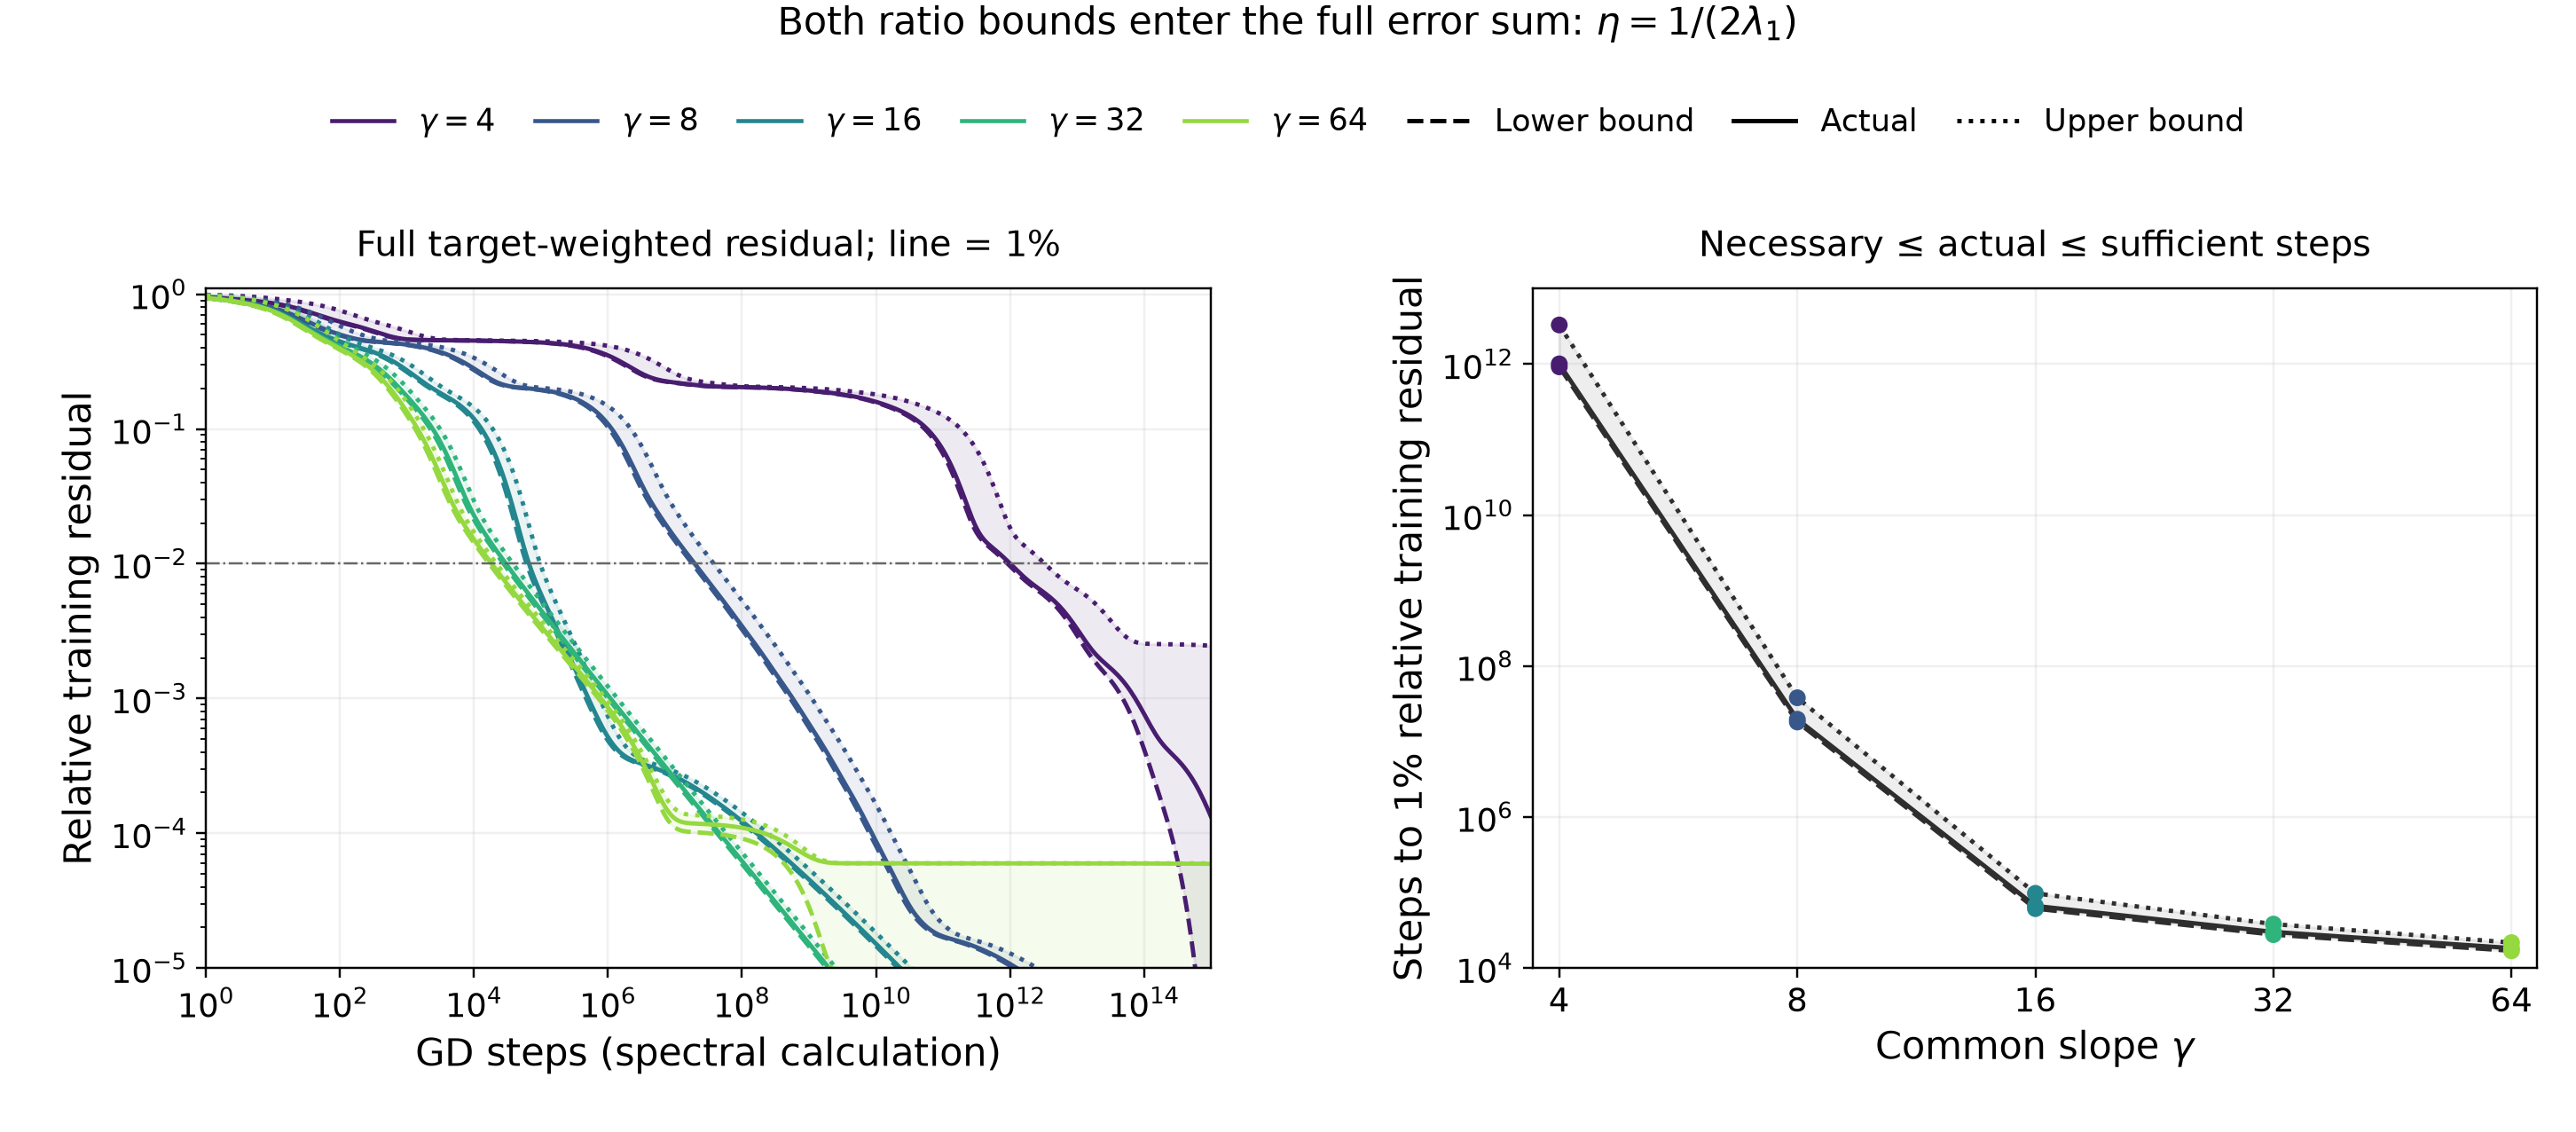
\includegraphics[width=\linewidth]{figures/full_residual_and_steps.png}
\caption{The finite-kernel spectral error, lower error curve using upper ratio endpoints, and upper error curve using lower endpoints. The 1\% threshold determines the step-count interval. Every curve is calculated by eigendecomposition and scalar powers; no long gradient descent run was executed. The bound curves use the actual target projections and the interval theorem, rather than a separate integral-kernel forecast. Appendix F documents numerical allowances and unresolved target energy.}
\end{figure}

\begin{center}\small\begin{tabularx}{\linewidth}{lXXX}
\toprule
\(\gamma\) & Necessary steps & Finite-kernel spectral steps & Sufficient steps \\
\midrule
4 & \(9.20\times10^{11}\) & \(1.008\times10^{12}\) & \(3.31\times10^{12}\) \\
8 & 18,111,765 & 19,697,563 & 37,941,446 \\
16 & 60,905 & 66,209 & 97,172 \\
32 & 27,547 & 29,938 & 38,036 \\
64 & 16,814 & 18,272 & 21,611 \\
\bottomrule\end{tabularx}\end{center}

The gamma-4 bound endpoints are rounded outward. These are checked floating-point evaluations of (11)--(12) with the numerical allowances in Appendix F, not certified bounds for the exact tanh kernel or guarantees for a floating-point gradient descent implementation. The necessary bound at gamma 4 is about 91\% of the finite-kernel spectral count; the sufficient bound is about 3.3 times that count.

At gamma 4, a separately computed readout achieves relative error \(5.85\times10^{-4}\), below the requested 1\%. Thus the long delay is not caused by that tolerance being unrepresentable. The high accuracy exists at the same geometry; ordinary readout gradient descent needs an impractical number of steps to obtain even the much weaker 1\% fit. At the larger tested gammas the relevant ratio intervals increase and the necessary and sufficient step counts decrease substantially. Appendix E extends the necessary-delay argument to stable scalar gradient descent schedules.

\clearpage\appendix
\section{The center integral and its restriction}

For \(d=x_a-x_b\ne0\), the identity

\[
1-\tanh u\tanh v=\coth(u-v)(\tanh u-\tanh v)
\]

with \(u=\gamma(x_a-c)\), \(v=\gamma(x_b-c)\), gives

\[
\int_{\mathbb R}(1-g_{ab}(c))\,dc
=\coth(\gamma d)\int_{\mathbb R}
[\tanh(\gamma(x_a-c))-\tanh(\gamma(x_b-c))]dc
=2d\coth(\gamma d).
\]

The difference of tanhs is integrable, and its log-cosh antiderivative gives \(2d\). At zero separation, the integral is that of \(\operatorname{sech}^2\), giving \(2/\gamma\). Splitting the whole-line deficit into \(I_c\) and its complement proves (5). The cell length \(Wh\), including half a cell beyond each outer center, is required for its constant term.

For any \(u\) with \(\mathbf1^\top u=0\), the constant part of (5) vanishes. In the finite double sum,

\[
\int_{\mathbb R}\left|\sum_a u_a\tanh(\gamma(x_a-c))\right|^2dc
=-2\sum_{a,b}u_a u_b d_{ab}\coth(\gamma d_{ab}).
\]

One can obtain this equality by integrating the products minus one; all these deficits are integrable, and the constant coefficients sum to zero. Substitution \(u=Qv\) yields \(H_\gamma=Q^\top K_\gamma^{(0)}Q\), proving the explicit formula used to construct the integral matrix.

The full matrix \(K_\gamma^{(0)}\) need not be positive semidefinite; \(H_\gamma\) is, by its integral definition. The entrywise nonnegative halo-deficit matrix in (5) need not be positive semidefinite either. The positive omitted-center matrix used in (8) is a different object: it is a sum of projected feature outer products on the lattice. The proof below uses that outer-product sign, not an entrywise sign assumption.

\section{Fourier identity and gamma dependence}

The cumulative integral of \(\rho_\gamma^{\mathrm{av}}\) is \((1+\tanh(\gamma x))/2\), proving the step-convolution identity. Substituting \(s=e^{2\gamma x}\) in its transform, with \(\nu=\omega/(2\gamma)\), gives

\[
\widehat{\rho_\gamma^{\mathrm{av}}}(\omega)
=\int_0^\infty\frac{s^{-i\nu}}{(1+s)^2}ds
=\Gamma(1-i\nu)\Gamma(1+i\nu)
=\frac{\pi\nu}{\sinh(\pi\nu)}.
\]

The middle equality is the beta integral and the last follows from the gamma reflection identity. The value at zero follows by continuity. For \(z>0\), \(d\log(z/\sinh z)/dz=1/z-\coth z<0\); since \(z\) decreases as gamma increases, \(M_\gamma\) increases.

For \(u=Qv\), the step combination \(g_{\mathrm{step}}(c)=\sum_a u_a\operatorname{sgn}(c-x_a)\) is compactly supported because \(\sum_a u_a=0\). Its derivative is \(2\sum_a u_a\delta_{x_a}\). Thus, away from zero,

\[
\widehat g_{\mathrm{step}}(\omega)
=\frac{2}{i\omega}\sum_a u_a e^{-i\omega x_a},
\qquad
\widehat g_\gamma=M_\gamma\widehat g_{\mathrm{step}}.
\]

The Fourier numerator vanishes at zero, and Parseval gives (7). No transform of a lone nondecaying tanh is needed. The two-input kernel identity in the main text can separately be understood as a tempered-distribution identity; it follows by applying the averaging density in each input.

For \(\gamma_b\ge\gamma_a\), subtracting (7) at the two gammas gives a nonnegative integral for every \(v\). Hence \(H_{\gamma_b}-H_{\gamma_a}\succeq0\). Courant--Fischer then proves the ordering of their eigenvalues without differentiating or tracking eigenvectors. This order applies to the integral matrices. It does not discard the finite corrections or the normalization in (10).


\subsection{An exact finite gamma change in each Fourier contribution}

For \(z=\pi|\omega|/(2\gamma)\), the double-angle identity gives
\[
\frac{M_{2\gamma}(\omega)}{M_\gamma(\omega)}
=\frac{(z/2)/\sinh(z/2)}{z/\sinh z}
=\frac{\sinh z}{2\sinh(z/2)}=\cosh(z/2).
\]
Squaring proves (7a). For a nonzero vector \(v\) with \(v^\top H_\gamma v>0\), define precisely
\[
w_{\gamma,v}(\omega)=
\frac{2}{\pi hm\,v^\top H_\gamma v}
\frac{M_\gamma(\omega)^2}{\omega^2}
\left|\sum_a(Qv)_ae^{-i\omega x_a}\right|^2.
\tag{B1}
\]
It is nonnegative and integrates to one by (7). Substituting (7a) inside the integral proves (7b). For example, if a fraction \(s\) of this density lies at \(|\omega|\ge\Omega\), then
\[
\frac{v^\top H_{2\gamma}v}{v^\top H_\gamma v}
\ge 1+s\left[\cosh^2\!\left(\frac{\pi\Omega}{4\gamma}\right)-1\right].
\tag{B2}
\]
Here \(s=\int_{|\omega|\ge\Omega}w_{\gamma,v}\); it is not determined by the eigenvalue rank. This is a rigorous statement of how a high-frequency contribution forces a larger gain. An upper bound from a low-frequency support condition is also immediate, but finite sums of sample exponentials are not generally bandlimited, so that condition should not be assumed for them.

\subsection{Why changing eigenvectors do not invalidate the local calculation}

Differentiating the multiplier yields
\[
\frac{\partial\log M_\gamma(\omega)^2}{\partial\log\gamma}
=2(z\coth z-1).
\tag{B3}
\]
This is zero at zero frequency. Its derivative with respect to \(z>0\) is
\(2(\coth z-z\operatorname{csch}^2z)>0\), because
\(\sinh z\cosh z>z\). Taylor expansion gives
\[
2(z\coth z-1)=\tfrac23z^2+O(z^4)
\quad(z\to0),\qquad
2(z\coth z-1)=2z-2+O(ze^{-2z})
\quad(z\to\infty).
\]
Differentiation under the integral in (7) is justified on every compact interval of positive gamma by the exponentially decaying multiplier and its derivative. It follows that
\[
\frac{\gamma v^\top H_\gamma'v}{v^\top H_\gamma v}
=\int 2(z\coth z-1)w_{\gamma,v}(\omega)\,d\omega.
\tag{B4}
\]
For a differentiable simple eigenpair \(H_\gamma v_i=\lambda_i(H_\gamma)v_i\), \(\|v_i\|=1\), differentiate and left-multiply by \(v_i^\top\):
\[
v_i^\top H_\gamma'v_i+\lambda_i(H_\gamma)v_i^\top v_i'
=\lambda_i(H_\gamma)'+\lambda_i(H_\gamma)v_i^\top v_i'.
\]
The eigenvector terms cancel. Using \(v_i^\top H_\gamma v_i=\lambda_i(H_\gamma)\) in (B4) proves (7c). At a repeated eigenvalue, use the eigenvalue branches obtained by diagonalizing \(H_\gamma'\) on the repeated eigenspace; an arbitrarily chosen eigenvector need not supply a derivative of an ordered branch. The matrix-order result remains valid without this differentiability qualification.

\subsection{Exact accounting for the actual finite normalized eigenvalues}

Embed the integral in sample space and keep everything else explicitly:
\[
\mathcal H_\gamma=QH_\gamma Q^\top,\qquad
\mathcal E_\gamma=K_\gamma-\mathcal H_\gamma.
\]
The latter matrix contains the mean direction and its coupling, the finite lattice, and the omitted center tails. For an actual unit eigenvector \(u_i\), let
\[
D_i=u_i^\top\mathcal H_\gamma u_i.
\]
When \(D_i>0\), define \(w_i\) by (B1) using \(v=Q^\top u_i\); this automatically subtracts the mean of \(u_i\). Apply the eigenvalue derivative identity to the full matrix \(K_\gamma\) first and then split its derivative. For simple positive eigenvalues, the exact result is
\[
\boxed{
\begin{aligned}
\frac{d\log(\lambda_i/\lambda_1)}{d\log\gamma}
={}&\frac{D_i}{\lambda_i}
\int 2(z\coth z-1)w_i(\omega)\,d\omega\\
&+\frac{\gamma u_i^\top\mathcal E_\gamma'u_i}{\lambda_i}
-\frac{\gamma u_1^\top K_\gamma'u_1}{\lambda_1}.
\end{aligned}}
\tag{B5}
\]
The first term is the Fourier contribution; the second is the exact finite-model correction; the third is the largest eigenvalue's fractional growth. In particular, a large first term only proves ratio growth after the other terms have been controlled. Differentiating \(D_i(\gamma)\) directly would incorrectly add eigenvector-motion terms to the first term. In (B5) they have already canceled in differentiating the actual eigenvalue.

There is no unknown function in the correction: \(\mathcal E_\gamma'=K_\gamma'-QH_\gamma'Q^\top\), with
\[
K_\gamma'=B_\gamma'B_\gamma^\top+B_\gamma(B_\gamma')^\top,
\quad (B_\gamma')_{aj}=\frac{(x_a-c_j)\operatorname{sech}^2(\gamma(x_a-c_j))}{\sqrt m},
\quad (B_\gamma')_{a0}=0,
\]
and \(H_\gamma'\) is given by (B3)--(B4). The saved diagnostics additionally separate the finite-center integral, mean coupling, and lattice difference. These calculations explain the observed mechanism; they are not a claim to predict all eigendirections without solving a matrix.

At gamma 16 in the saved \(W=153,m=263\) geometry, the checked quantities are:
\begin{center}\small
\begin{tabular}{rrrr}
\toprule
Full rank & Fourier average in (B5) & \(d\log\lambda_i/d\log\gamma\) & \(d\log\rho_i/d\log\gamma\)\\
\midrule
2  & 0.01463423 & 0.01463424 & 0.00367337\\
6  & 0.35105663 & 0.35105679 & 0.34009592\\
12 & 1.48709604 & 1.48709713 & 1.47613626\\
20 & 3.54684319 & 3.54684847 & 3.53588761\\
32 & 6.90227140 & 6.90229545 & 6.89133459\\
\bottomrule
\end{tabular}
\end{center}
The Fourier-average column is \(\int 2(z\coth z-1)w_i\); it omits \(D_i/\lambda_i\) and the correction term, rather than defining them away. The largest eigenvalue's growth is 0.010960864. The small differences shown are measured facts of these modes at this gamma. At gamma 8, mean coupling is not negligible for every low mode, and the full correction accounting is required.

The existing calculation also integrates the Fourier estimate along the actual changing eigendirections. From gamma 8 to 16, the observed ratio gains at ranks 12, 20, and 32 are respectively 5.9814, 49.2169, and 1277.7239. The integrated Fourier estimate with corrections omitted gives 5.9790, 49.1050, and 1263.3445. This agreement supports the explanation in the studied regime. It is a diagnostic of the mechanism, not an independent guarantee about the unknown eigenvectors or a new definition of the absolute interval theorem.

Most importantly, bounds on the values of correction matrices are not bounds on their derivatives. One may not differentiate \(\|R_\gamma\|\le\delta_\gamma\) or \(0\preceq T_{\mathrm{tail},\gamma}\preceq\tau_\gamma I\) to justify (B5)'s sign. The note uses the exact derivative accounting for this diagnostic and the finite-value interval test (10a) for a proved comparison between gammas.

\section{Analytic corrections for the lattice and the finite halo}

Write the center lattice as \(c_0+h\mathbb Z\). For the zero-mean restriction, the infinite lattice sum converges. The finite sum equals that infinite sum minus the absent centers. The bias vanishes under \(Q\).

\subsection{Explicit lattice terms}

Define the integrable product deficit

\[
F_{ab}(c)=\tanh(\gamma(x_a-c))\tanh(\gamma(x_b-c))-1.
\]

For \(\nu\ne0\), its Fourier transform is

\[
\widehat F_{ab}(\nu)
=-\frac{4M_\gamma(\nu)}{\nu}
\sin(\nu d_{ab}/2)\coth(\gamma d_{ab})
e^{-i\nu(x_a+x_b)/2}.
\tag{C1}
\]

The diagonal limit is \(-2M_\gamma(\nu)e^{-i\nu x_a}/\gamma\). The identity follows by expressing the product minus one as a coth factor times the difference of two tanhs, then transforming the integrable difference. Pairing positive and negative lattice frequencies \(\nu_k=2\pi k/h\) gives real symmetric corrections

\[
G_{\gamma,k}=\frac2{hm}Q^\top
\operatorname{Re}\!\left[e^{i\nu_k c_0}\widehat F(\nu_k)\right]Q,
\qquad G_\gamma=\sum_{k=1}^{p}G_{\gamma,k}.
\tag{C2}
\]

The truncation count \(p\ge0\) is a computational choice, not target energy. Individual correction matrices need not be positive semidefinite. Their gamma dependence is explicit in (C1), including the multiplier at each lattice frequency.

\subsection{Bound on unretained lattice terms}

Choose any \(0<\vartheta<\pi/2\) and let \(d=\vartheta/\gamma\). For a real zero-mean vector \(u\), write \(g(c)=\sum_a u_a\tanh(\gamma(c-x_a))\), and \(\bar x=m^{-1}\sum_a x_a\). On the two boundaries of the analytic strip,

\[
\int_{\mathbb R}|g(t\pm id)|^2dt
\le\frac{4\gamma}{3}\sec^4\vartheta\,
\|x-\bar x\mathbf1\|^2\|u\|^2.
\tag{C3}
\]

To see the constant, use \(\sum u_a=0\) to subtract \(\tanh(\gamma(c-\bar x))\) from every term, express each difference as an integral of the derivative, and apply Minkowski and Cauchy--Schwarz. The derivative has squared \(L_2\) norm at most \((4\gamma/3)\sec^4\vartheta\), because \(|\operatorname{sech}^2(t+i\vartheta)|\le\sec^2\vartheta\operatorname{sech}^2t\) and \(\int\operatorname{sech}^4t\,dt=4/3\).

Contour shifting applies to the analytic function \(g(z)^2\), not to \(|g(z)|^2\). Equation (C3) bounds the shifted absolute integral, so its Fourier transform decays as \(e^{-d|\nu|}\). Poisson summation and a geometric series over the unretained indices \(k>p\) give the operator-norm allowance

\[
\boxed{
\delta_\gamma=
\frac{8\gamma\|x-\bar x\mathbf1\|^2\sec^4\vartheta}
{3hm\,[e^{2\pi\vartheta/(\gamma h)}-1]}
e^{-2\pi\vartheta p/(\gamma h)}.
}
\tag{C4}
\]

This is uniform over unit vectors in the restricted space. In the calculation, \(\vartheta=\arctan(\pi/(2\gamma h))\), and enough explicit terms are retained to make (C4) at most \(10^{-18}\). The allowance concerns uncomputed terms, not floating-point evaluation error.

\subsection{Exterior centers and the matrix enclosure}

Let \(\mathcal F\) be a finite collection of absent lattice centers, and retain their contribution

\[
T_\gamma=\frac1m\sum_{c\in\mathcal F}
Q^\top t_\gamma(c)t_\gamma(c)^\top Q.
\]

Include all absent centers inside the sample range. Suppose the unretained centers begin at \(c_R>x_{\max}\) and \(c_L<x_{\min}\). The inequality \(1-\tanh t\le2e^{-2t}\) for \(t\ge0\), cancellation of the constant vectors under \(Q\), and summation over the two exterior lattice tails give

\[
0\preceq T_{\mathrm{tail},\gamma}\preceq\tau_\gamma I,
\qquad
\tau_\gamma=
\frac{4[e^{-4\gamma(c_R-x_{\max})}+e^{-4\gamma(x_{\min}-c_L)}]}
{1-e^{-4\gamma h}}.
\tag{C5}
\]

For example, each right-tail projected outer product has norm at most \(4e^{-4\gamma(c-x_{\max})}\) after the factor \(1/m\); the geometric series gives its contribution to (C5). The implementation retains \(\lceil18/(\gamma h)\rceil\) absent centers on each side of the finite network.

Poisson summation gives the infinite lattice matrix as \(H_\gamma+G_\gamma+R_\gamma\), where \(\|R_\gamma\|_2\le\delta_\gamma\). Subtracting all absent centers therefore gives exactly

\[
Q^\top K_\gamma Q
=S_\gamma+R_\gamma-T_{\mathrm{tail},\gamma}.
\]

This proves (9). All quantities are evaluated at the same gamma. The retained corrections may be substantial; it is their unretained remainder that must be bounded. A small global error relative to the largest eigenvalue is not enough when studying a much smaller eigenvalue.


\subsection{How the corrected eigenvalues and remainder bounds depend on gamma}

The dependence of \(\beta_i\) is completely specified by
\[
\beta_i(\gamma)=\lambda_i\left(
-\frac{2}{hm}Q^\top[d_{ab}\coth(\gamma d_{ab})]Q
+\sum_{k=1}^{p}G_{\gamma,k}
-\frac1m\sum_{c\in\mathcal F}Q^\top t_\gamma(c)t_\gamma(c)^\top Q
\right).
\tag{C6}
\]
The diagonal \(d\coth(\gamma d)\) is interpreted as \(1/\gamma\). The samples, lattice spacing, phase \(c_0\), and retained sets are known. No measured actual small eigenvalue enters (C6).

For fixed truncation counts and sets, all entries in (C6) are smooth for \(\gamma>0\). Their derivatives are explicit. For example,
\[
(H_\gamma')=\frac{2}{hm}Q^\top
[d_{ab}^2\operatorname{csch}^2(\gamma d_{ab})]Q,
\]
with diagonal value \(1/\gamma^2\) in the bracket, and
\[
T_\gamma'=\frac1m\sum_{c\in\mathcal F}Q^\top
[t_\gamma'(c)t_\gamma(c)^\top+t_\gamma(c)t_\gamma'(c)^\top]Q,
\quad (t_\gamma'(c))_a=(x_a-c)\operatorname{sech}^2(\gamma(x_a-c)).
\]
For the lattice terms, differentiate (C1)--(C2), using
\(\partial_\gamma M_\gamma(\nu)=M_\gamma(\nu)(z_\nu\coth z_\nu-1)/\gamma\),
where \(z_\nu=\pi|\nu|/(2\gamma)\), and
\(\partial_\gamma\coth(\gamma d)=-d\operatorname{csch}^2(\gamma d)\).
For a simple eigenpair \(S_\gamma v_i=\beta_i v_i\), with \(\|v_i\|=1\),
\[
\beta_i'=v_i^\top(H_\gamma'+G_\gamma'-T_\gamma')v_i.
\tag{C7}
\]
Although \(H_\gamma'\succeq0\), the last two terms do not have an automatic favorable sign. Thus (C6) specifies the gamma dependence; it is not a universal monotonicity theorem for \(\beta_i\). Changing truncation counts can also introduce harmless changes in the approximate matrix; the enclosure remains valid pointwise on both sides of such a change.

For fixed \(\vartheta\) and \(p\), put \(b=2\pi\vartheta/h\). Formula (C4) is proportional to
\(\gamma e^{-bp/\gamma}/(e^{b/\gamma}-1)\), whose logarithmic derivative is
\[
1+\frac{b/\gamma}{1-e^{-b/\gamma}}+\frac{bp}{\gamma}>0.
\]
This proves the claimed increase of the lattice remainder bound at fixed truncation. It describes the scalar allowance, not the derivative of the remainder matrix. Formula (C5) decreases with gamma when the first unretained centers are fixed: its numerator decreases and its denominator increases. Choosing counts adaptively keeps these allowances small without changing the physical center set of the network.

The actual truncations in the saved selected-rank calculation were:
\begin{center}\small
\begin{tabular}{rrrrr}
\toprule
\(\gamma\) & Lattice pairs \(p\) & Exterior centers per side & \(\delta_\gamma\) & \(\tau_\gamma\)\\
\midrule
4  & 0 & 288 & \(1.31\times10^{-59}\) & \(7.54\times10^{-32}\)\\
8  & 0 & 144 & \(3.21\times10^{-26}\) & \(1.64\times10^{-33}\)\\
16 & 1 & 72  & \(2.15\times10^{-25}\) & \(1.54\times10^{-36}\)\\
32 & 3 & 36  & \(5.93\times10^{-23}\) & \(2.54\times10^{-42}\)\\
64 & 8 & 18  & \(9.80\times10^{-21}\) & \(1.14\times10^{-53}\)\\
\bottomrule
\end{tabular}
\end{center}
These are existing floating-point evaluations of the analytic expressions. Their smallness does not say that \(G_\gamma\) or \(T_\gamma\) themselves are small: those retained corrections were already included in \(\beta_i\). Nor does it eliminate floating-point and quadrature error, which Appendix F treats separately. At these ranks, the one-index interlacing and largest-eigenvalue enclosure can account for much more interval width than delta and tau.

\section{Eigenvalue endpoints and normalization}

Let \(\kappa_1\ge\cdots\ge\kappa_{m-1}\) be the eigenvalues of \(Q^\top K_\gamma Q\). Weyl's order inequalities applied to (9) give

\[
\beta_i-\delta_\gamma-\tau_\gamma\le\kappa_i\le\beta_i+\delta_\gamma.
\]

Compression interlacing gives \(\lambda_i\ge\kappa_i\ge\lambda_{i+1}\). Combining the lower inequality at index \(i\) and the upper inequality at index \(i-1\) proves (10). For the last full eigenvalue, only the upper interlacing inequality is available; nonnegativity supplies its lower bound. Since \(\operatorname{rank}B_\gamma\le W+1\), all indices \(i>W+1\) are exact zeros, if such indices exist. Numerically small positive singular values are not thereby exact zeros.

For the largest eigenvalue, set \(e=\mathbf1/\sqrt m\). Its Rayleigh quotient supplies

\[
\ell_\gamma=e^\top K_\gamma e
=\|B_\gamma^\top e\|^2
=1+\sum_j\left[\frac1m\sum_a\tanh(\gamma(x_a-c_j))\right]^2.
\tag{D1}
\]

In the orthonormal basis \([e,Q]\), the kernel has blocks \(\bigl(\begin{smallmatrix}\ell_\gamma&b_{\rm vec}^\top\\b_{\rm vec}&Q^\top K_\gamma Q\end{smallmatrix}\bigr)\), where \(b_{\rm vec}=Q^\top B_\gamma(B_\gamma^\top e)\). Put \(b=\|b_{\rm vec}\|\) and \(c=\beta_1+\delta_\gamma\). Bounding the cross term by \(b\) and the restricted block by \(cI\) yields

\[
L_\gamma=
\frac{\ell_\gamma+c+\sqrt{(\ell_\gamma-c)^2+4b^2}}2
\ge\lambda_1(K_\gamma).
\tag{D2}
\]

This is the largest eigenvalue of a two-by-two scalar matrix. Equations (D1)--(D2) use finite-feature matrix-vector products and the corrected integral spectrum. They do not use the actual finite small eigenvalues. The actual feature SVD is used separately to compare the bounds and to obtain the target weights for Section 4. Coarser universal bounds follow from the bias and trace: \(1\le\lambda_1\le W+1\).


\subsection{Why the normalization can saturate while small modes still grow}

For a center outside the sample interval at distance \(d_j>0\), every feature value has the same sign and magnitude at least \(\tanh(\gamma d_j)\). Consequently
\[
\ell_\gamma\ge1+\sum_{j:\,c_j\notin[x_{\min},x_{\max}]}
\tanh^2(\gamma d_j).
\tag{D3}
\]
This proves a structural lower bound from the bias and saturated exterior features. To conclude it is proportional to width would additionally require a proportional number of suitably distant centers; a square-root halo alone does not give that conclusion. The sharper quantity (D1) uses all feature means.

For finite fixed samples and centers, set \(s_{aj}=\operatorname{sgn}(x_a-c_j)\), with \(\operatorname{sgn}(0)=0\), and let
\(\bar s_j=m^{-1}\sum_a s_{aj}\). Then
\[
\ell_\infty=1+\sum_j\bar s_j^2,
\qquad
|\ell_\gamma-\ell_\infty|
\le\frac4m\sum_{a,j:\,x_a\ne c_j}e^{-2\gamma|x_a-c_j|}.
\tag{D4}
\]
Indeed, \(|\tanh t-\operatorname{sgn}t|\le2e^{-2|t|}\) for nonzero \(t\); coincident pairs have exactly zero difference. Average over samples and use \(|a^2-b^2|\le2|a-b|\) for \(|a|,|b|\le1\). This gives an explicit limit of the feature-mean normalization, rather than an unexplained assertion that the top eigenvalue is fixed.

The largest eigenvalue itself also converges to that of the step-feature matrix. Let \(B_\infty\) have the same bias and entries \(s_{aj}/\sqrt m\), and define
\[
\varepsilon_\gamma^{\mathrm{step}}
=\frac2{\sqrt m}\left(\sum_{a,j:\,x_a\ne c_j}
 e^{-4\gamma|x_a-c_j|}\right)^{1/2}.
\]
The feature difference has Frobenius norm at most \(\varepsilon_\gamma^{\mathrm{step}}\). Since both feature matrices have operator norm at most \(\sqrt{W+1}\),
\[
|\lambda_1(K_\gamma)-\lambda_1(K_\infty)|
\le\|K_\gamma-K_\infty\|_2
\le2\sqrt{W+1}\,\varepsilon_\gamma^{\mathrm{step}}.
\tag{D5}
\]
These are valid asymptotic statements. Small sample--center separations can make (D4)--(D5) loose at the moderate gammas of interest, so they are not used as precision bounds in the figures. In that range the explicit finite normalization interval (D1)--(D2), and its saved values, quantify the denominator:
\begin{center}\small
\begin{tabular}{rrrr}
\toprule
\(\gamma\) & \(\ell_\gamma\) & Actual \(\lambda_1\) & \(L_\gamma\)\\
\midrule
4 & 63.1963 & 68.4813 & 74.6609\\
8 & 66.8232 & 72.6740 & 79.3592\\
16 & 67.9418 & 73.8587 & 80.6028\\
32 & 68.2403 & 74.1636 & 80.9136\\
64 & 68.3161 & 74.2402 & 80.9910\\
\bottomrule
\end{tabular}
\end{center}
Thus the numerator and denominator are both accounted for. There is no theorem that saturation makes every normalized eigenvalue monotone: the step limit can lose directions, as the counterexample below shows. What is established for the displayed finite comparisons is the separation of their ratio intervals.

\section{What the training bounds imply, and what they do not}

\subsection{Error bounds and threshold crossings}

For every index, \(0\le\underline\rho_i\le\rho_i\le\overline\rho_i\le1\). Multiplying the corresponding scalar inequalities by nonnegative \(p_i\) and summing proves (11). All three curves are nonincreasing in \(n\), so the first crossing of the lower curve cannot be later than the actual crossing, and the first crossing of the upper curve cannot be earlier. This proves (12), including empty-set cases.

Omitting nonnegative terms preserves a lower error bound. It does not preserve an upper error bound. If some component is unresolved, assigning it lower rate zero retains its full weight in the upper curve. Exact zero-eigenvalue components have factor one in the actual curve; they must not be confused with unresolved positive eigenvalues. Repeated eigenvalues cause no ambiguity in the actual curve because the sum of weights in their eigenspace is basis-independent.

A compact necessary-time test does not require the full error curve. Let \(P_i^+=\sum_{j\ge i:\lambda_j>0}p_j\), the target's squared-norm fraction in positive-eigenvalue directions at ranks \(j\ge i\). Ordering gives \(\rho_j\le\rho_i\le\overline\rho_i\), and hence

\[
E_\gamma(n)^2\ge P_i^+(1-\overline\rho_i/2)^{2n}.
\]

If \(P_i^+>\epsilon^2\) and \(\overline\rho_i>0\), attaining tolerance requires

\[
n_\epsilon\ge
\left\lceil
\frac{\log(\sqrt{P_i^+}/\epsilon)}{-\log(1-\overline\rho_i/2)}
\right\rceil.
\tag{E1}
\]

More generally, a known lower bound on \(P_i^+\), or the energy of any subset of these positive directions, gives a valid necessary-time bound. Positivity matters for the interpretation: \(u_j=B_\gamma(B_\gamma^\top u_j/\lambda_j)\) when \(\lambda_j>0\), so that component is representable. The theorem does not supply the target weights from gamma alone.

\subsection{Scalar learning-rate schedules}

Keep the same frozen kernel, but allow \(0\le\eta_t\le2/\lambda_1\) at every step. If a selected positive band has ratios at most \(b<1/2\), then \(1-\eta_t\lambda_j\ge1-2b>0\). A target energy fraction \(P\) in that band therefore gives

\[
E(n)^2\ge P(1-2b)^{2n},
\qquad
n_\epsilon\ge
\left\lceil\frac{\log(\sqrt P/\epsilon)}{-\log(1-2b)}\right\rceil
\quad(P>\epsilon^2).
\]

For small \(b\), allowing this schedule weakens the displayed necessary-time lower bound by approximately a factor of four compared with \(\eta=0.5/\lambda_1\). This is a comparison of the lower bounds, not a general theorem about the ratio of actual crossing times. It does not cover steps outside the stated per-update stability range, momentum, or matrix preconditioning.

These results concern frozen geometry and Euclidean readout gradient descent, not Adam, preconditioned readout coordinates, or the joint dynamics of gamma.

\subsection{Why the theorem does not claim universal ratio monotonicity}

Take samples \((-1,1)\), centers \((-3/2,0,3/2)\), and the bias. Both sets are uniform and symmetric. Put \(a=\tanh(5\gamma/2)\), \(b=\tanh(\gamma/2)\). The even and odd eigenvalues of the normalized kernel are

\[
\lambda_+=1+\tfrac12(a+b)^2,
\qquad
\lambda_-=\tanh^2\gamma+\tfrac12(a-b)^2,
\qquad\lambda_+>\lambda_-.
\]

As \(\gamma\to\infty\),

\[
\frac{\lambda_-}{\lambda_+}
=\frac13+\frac49e^{-\gamma}+O(e^{-2\gamma}).
\]

The ratio eventually decreases. Thus a universal assertion that increasing gamma always improves every finite ratio would be false. The note instead provides absolute bounds at each gamma and demonstrates disjoint intervals and faster spectral convergence in the specified regimes. Its small-gamma budget obstruction does not require that stronger assertion.

\section{Numerical calculations and reproducibility}

\subsection{Geometry, target, and scope}

The calculations use \(N=128\) equal intervals on \([-1,1]\), \(h=2/N\), \(N+1=129\) interior centers, and \(\lceil\sqrt N\rceil=12\) halo centers per side. There are \(W=153\) tanh neurons and one bias feature. The 263 samples include both endpoints and are equally spaced. The center lattice runs from \(-1.1875\) to \(1.1875\). Every gamma uses the same samples, centers, target, and raw readout parameterization. The learning rate is normalized separately by each actual \(\lambda_1\).

The selected-rank plot reuses 33 logarithmically spaced gammas from 4 to 64, at ranks 13, 20, 26, and 33, including both symmetry classes. The full error and time intervals are evaluated at gamma 4, 8, 16, 32, and 64. The mixed-sine target is the one stated in Section 4. The result concerns training error, not a claim about error between samples.

\subsection{Computation and numerical allowances}

The integral matrix is evaluated through a positive quadrature feature factor, using piecewise Gauss--Legendre quadrature. Its SVD supplies a basis in which the integral spectrum is diagonal; the explicit lattice corrections and omitted-center outer products are added in that basis. This avoids subtracting nearly equal large entries before resolving small eigenvalues. The finite-feature singular values are squared to obtain the actual eigenvalues, rather than diagonalizing a rounded Gram matrix.

The exact theorem uses the whole-line \(H_\gamma\). Truncating its integration domain at \(\max_a|x_a|+P/\gamma\) omits a positive matrix with norm at most \(2e^{-4P}/(h\gamma)\). The implementation adds that allowance to upper eigenvalue endpoints and the upper normalization. The exterior lattice remainder is separately controlled by (C5).

The analytic allowances do not include quadrature or floating-point error. Figure 2 shows the original selected-rank evaluations, checked by increasing quadrature order from 10 to 16 and integration padding from 20 to 24, and by independent feature-SVD drivers. The maximum checked relative change in the selected corrected eigenvalues was \(5.8\times10^{-8}\); actual finite-feature eigenvalues agreed to \(7.2\times10^{-12}\) relative at those ranks. Those are numerical checks, not certified bounds on every rounding error.

For the full error curves, add a numerical allowance \(\nu_\gamma=64\epsilon_{64}\|S_\gamma\|_2\), where \(\epsilon_{64}\) is double-precision machine epsilon. Subtract it from lower eigenvalue numerators; add it to upper numerators and the restricted-block upper bound in (D2). This empirical allowance is checked against independent refinement, not proved to enclose every rounding error. It prevents numerical positive eigenvalues near the precision limit from supporting unjustified positive lower rates.

Actual feature-SVD ratios above \(10^{-18}\) are retained as numerically resolved. Every other mode receives zero lower rate and keeps its full energy in the upper error curve. The lower curve drops both the unresolved-mode energy and the computed projection remainder outside the returned finite-feature singular vectors. The upper curve retains both. The projection remainder is recorded separately from unresolved positive-mode energy; neither numerical split is used to certify the true asymptotic nullspace floor.

At all five gammas, the guarded endpoints bracket every retained numerical ratio, and the full error curves bracket the finite-kernel spectral curve. Repeating the construction with quadrature order 16 and padding 24 changes the gamma-4 bound counts by less than \(8\times10^{-9}\) relatively; the other bound counts agree as integers. After changing basis, the corrected-matrix refinement discrepancy is below the chosen numerical allowance. Independent feature-SVD drivers also preserve the resolved-mode ordering and count intervals. The upper curves all cross 1\%; their nondecaying energy is explicitly retained, not discarded to force a finite crossing. The crossing search is capped at \(10^{18}\); no reported count hits that cap.

For very small rates, powers are evaluated as \(\exp(2n\log1p(-\rho/2))\). Integer crossing times use bracketing and binary search. These calculations evaluate the frozen-kernel recurrence in exact-arithmetic form from computed spectral data; trillion-step counts do not imply that trillion-step floating-point training was executed or verified.

\subsection{Proven statements and numerical evidence}

\begin{center}\small\begin{tabularx}{\linewidth}{p{0.35\linewidth}X}
\toprule
Statement & Status \\
\midrule
gradient descent recurrence and target-weighted error formula & Exact for the specified frozen-feature updates and zero initial readout. \\
Integral decomposition, Fourier identity, and ordered growth of \(H_\gamma\) & Proved under the stated definitions; no Fourier-eigenvector assumption. \\
Corrected finite ratio interval & Proved with analytic lattice and exterior-center allowances. \\
Error sandwich, first-crossing interval, and positive-tail delay & Proved using the same actual target weights or justified energy bounds. \\
Evaluated intervals, attainable readouts, and step-count numbers & Checked floating-point results; no directed-rounding certificate. \\
Every finite ratio or target crossing improves with gamma & Not claimed; universal ratio monotonicity is false. \\
\bottomrule\end{tabularx}\end{center}

\subsection{Provenance and relation to the paper draft}
This edition expands the four-part argument and proof appendices from the revision-4 gamma-ratio note (23 September 2026), retaining its interval theorem and existing figures. The revision makes the multiplier gain, corrected spectrum, analytic remainders, and normalization dependence explicit. The added mechanism tables are recovered from the existing spectrum-mechanism diagnostics; no new training was performed. Its two independent revision-4 reviews specify the treatment of target weights, unresolved modes, interlacing indices, and numerical allowances. The original sources are:
\begin{itemize}\raggedright
\item \path{docs/frozen_geometry_capacity_access/gamma_ratio_note/gamma_ratio_note_v4.md}; companion files \path{revision4_math_review.md} and \path{revision4_argument_review.md} in that directory.
\item The experiment sources \path{direct_ratio_interval.py} and \path{note_interval_figures.py} under \path{experiments/expD37_capacity_access_figures/gamma_solve/spectrum_mechanism/}.
\item Saved reports and figure manifests under the matching \path{results/checkpoint_D_optimizers/expD37_capacity_access_figures/gamma_solve/spectrum_mechanism/} directory, especially \path{direct_ratio_interval/}, \path{note_interval_figures/}, \path{data/summary.json}, \path{data/integrated_growth.json}, and \path{spectrum_mechanism_results.md}.
\end{itemize}
These are existing numerical results; this edition does not run new training. The example here has 153 hidden neurons, 263 samples, and a highest target frequency of $10\pi$. It is not the current paper's separate width-512, $14\pi$ example. The figure and step-count claims in this note should retain their own experimental configuration when reused.
\end{document}
